\chapter{Bipolar coordinates}
\label{ch:bipolar}

In this chapter
we apply boundary tracing to the conduction--radiation problem
starting from the known solution
to Laplace's equation~(\ref{eq:laplace-steady-conduction})
for equal and opposite line sources.
As before,
we determine traced boundaries along which
the radiation condition~(\ref{eq:radiation-boundary-condition}) holds
and use the convex portions to construct conduction--radiation domains.

\section{Known solution}
\label{sec:bipolar.known}

The problem at hand is best tackled using bipolar coordinates.
While it would be well to introduce the bipolar coordinate system
before writing down the known solution,
a better understanding of the physics is obtained
by first writing down the known solution
and then observing how bipolar coordinates arise as a result.

Suppose that the equal and opposite line sources
are the same strength as the line source~(\ref{eq:line-laplace-solution})
but located at~$(x, y) = (\pm a, 0)$.
Since the distance to each source is
\begin{equation}
  r_\pm = \sqrt{(x \mp a)^2 + y^2},
  \label{eq:bipolar-source-distances}
\end{equation}
the known solution is given by
\begin{equation}
  T =
    T_0 \log \roundbr*{\frac{r_0}{r_+}}
      -
    T_0 \log \roundbr*{\frac{r_0}{r_-}},
  \label{eq:bipolar-laplace-solution-terms}
\end{equation}
which reduces%
\footnote{
  The remarkable cancellation of the reference length~$r_0$
  occurs only for equal and opposite line sources.
}
to
\begin{important}{equation}
  T = T_0 \log \roundbr*{\frac{r_-}{r_+}}.
  \label{eq:bipolar-laplace-solution-source-distances}
\end{important}
This can be rewritten as
\begin{equation}
  T = T_0 \tanh^{-1} \roundbr*{\frac{2 a x}{x^2 + y^2 + a^2}},
  \label{eq:bipolar-laplace-solution-inverse-tanh}
\end{equation}
and the bipolar coordinate system~$(u, v)$ arises
from using the dimensionless quantity
\begin{equation}
  v
    = \frac{T}{T_0}
    = \tanh^{-1} \roundbr*{\frac{2 a x}{x^2 + y^2 + a^2}}
  \label{eq:v-transformation-bipolar}
\end{equation}
as the second coordinate,
so that $T$-contours are also $v$-contours,
and the known solution is simply given by
\begin{important}{equation}
  T = T_0 \cdot v.
  \label{eq:bipolar-laplace-solution}
\end{important}
By rearranging~(\ref{eq:v-transformation-bipolar}) and completing the square,
we see that the $T$-contours (and hence $v$-contours) are circles of the form
\begin{equation}
  (x - a \coth v)^2 + y^2 = a^2 \csch^2 v.
  \label{eq:bipolar-circle-v}
\end{equation}
Desiring an orthogonal coordinate system,
and knowing that a potential and its associated stream function
cross everywhere at right angles,
the other bipolar coordinate~$u$ is determined by computing
the harmonic conjugate of~$v$,
yielding the angular coordinate
\begin{equation}
  u = \tan^{-1} \roundbr*{\frac{2 a y}{x^2 + y^2 - a^2}}.
  \label{eq:u-transformation-bipolar}
\end{equation}
Here, the arctangent is to be returned in the quadrant corresponding to
an abscissa of~$x^2 + y^2 - a^2$ and an ordinate of~$2 a y$,
so that $u$~is reckoned modulo~$2 \pi$ rather than~$\pi$.

\subsection{Bipolar coordinates}
\label{sec:bipolar.known.coordinates}

Of course it is the forward transformation which is more useful,
and upon inverting~(\ref{eq:v-transformation-bipolar})
\&~(\ref{eq:u-transformation-bipolar})
we have
\begin{align}
  x &= \frac{a \sinh v}{\cosh v - \cos u},
    \label{eq:x-transformation-bipolar}
    \\[\tallspace]
  y &= \frac{a \sin u}{\cosh v - \cos u}.
    \label{eq:y-transformation-bipolar}
\end{align}
The length scale~$a$ is intrinsic to the coordinate system,
as it encodes the locations of the singularities~$(x, y) = (\pm a, 0)$.
The scale factors for the two coordinates turn out to be the same:
\begin{equation}
  \scalefac = \frac{a}{\cosh v - \cos u}.
  \label{eq:scale-factor-bipolar}
\end{equation}

\begin{figure}
  \centredfigurecontent[width=0.87\textwidth]{bipolar-coordinates}{
    Contours of the bipolar coordinates~$(u, v)$.
    The negative singularity~($v = -\infty$) is~$(x, y) = (-a, 0)$.
    The positive singularity~($v = +\infty$) is~$(x, y) = (+a, 0)$.
  }
\end{figure}

Figure~\ref{fig:bipolar-coordinates} shows the contours
of the two bipolar coordinates.
The $v$-contours are the non-intersecting circles~(\ref{eq:bipolar-circle-v})
which enclose the nearest singularity.
The limiting case~$v = -\infty$ corresponds to the negative singularity.
As $v$~increases the circular contour grows,
until~$v = 0$ where it coincides with the $y$-axis.
As $v$~waxes positive the circular contour shrinks,
becoming the positive singularity at~$v = +\infty$.

The equation~(\ref{eq:u-transformation-bipolar})
for the angular coordinate~$u$
may likewise undergo rearrangement and completion of the square
to become
\begin{equation}
  x^2 + (y - a \cot u)^2 = a^2 \csc^2 u.
  \label{eq:bipolar-circle-u}
\end{equation}
Despite this, the $u$-contours are \emph{not} full circles.
Since the arctangent in~(\ref{eq:u-transformation-bipolar})
is to be returned in the quadrant of~$(x^2 + y^2 - a^2, \, 2 a y)$,
the $u$-contours are in fact
only circular \emph{arcs} which terminate at the singularities
(Figure~\ref{fig:bipolar-u}),
with $u < \SI{180}{\degree}$~for arcs above the $x$-axis (i.e.~$y > 0$)
and $u > \SI{180}{\degree}$~for arcs below it (i.e.~$y < 0$).
Geometrically, $u$~is the angle on the underside of the two chords
from the two singularities.
Note that $u$~increases anticlockwise around the positive singularity
and clockwise around the negative singularity.

\begin{figure}
  \newcommand*{\subfigurewidth}{0.35\textwidth}
  \centering
  \hspace*{\fill}
  \begin{subfigure}[t]{\subfigurewidth}
    \centredfigurecontent{bipolar-u-less-than-pi}{%
      $u = \const < \SI{180}{\degree}$
    }
  \end{subfigure}
    \hfill
  \begin{subfigure}[t]{\subfigurewidth}
    \centredfigurecontent{bipolar-u-more-than-pi}{%
      $u = \const > \SI{180}{\degree}$
    }
  \end{subfigure}
  \hspace*{\fill}
  \caption{
    Circular arcs formed by curves of constant~$u$.
  }
  \label{fig:bipolar-u}
\end{figure}

\subsection{Scaling}
\label{sec:bipolar.known.scaling}

Since the length scale has already been fixed at~$a$,
we let
\begin{align}
  x &= a \scaled{x}, \label{eq:bipolar-x-scaling} \\
  y &= a \scaled{y}, \label{eq:bipolar-y-scaling}
\end{align}
so that
\begin{equation}
  \del = \scaleddel / a.
  \label{eq:bipolar-del-scaling}
\end{equation}
For the bipolar scale factor~$\scalefac$ it is sensible to put
\begin{equation}
  \scalefac = a \scaled{\scalefac}.
  \label{eq:bipolar-scale-factor-scaling}
\end{equation}
Also putting
\begin{equation}
  T = \Theta \scaled{T},
  \label{eq:bipolar-temperature-scaling}
\end{equation}
the radiation boundary condition~(\ref{eq:radiation-boundary-condition})
and the known solution~(\ref{eq:bipolar-laplace-solution})
become
\begin{align}
  \normalvec \dotp \scaleddel \scaled{T}
    &= -\group{c a \Theta^3} \scaled{T}^4,
    \label{eq:bipolar-scaled-radiation-boundary-condition-with-groups}
    \\[\tallspace]
  \scaled{T} &= \group{\frac{T_0}{\Theta}} v.
    \label{eq:bipolar-scaled-laplace-solution-with-groups}
\end{align}
Given two dimensionless groups but only one free scale~$\Theta$,
only one group can be set to unity,
and as in the polar case (Section~\ref{sec:polar.line.scaling})
we choose
\begin{equation}
  \Theta = T_0
    \label{eq:bipolar-temperature-scale}
\end{equation}
and define the dimensionless group
\begin{equation}
  A = \frac{1}{c a {T_0}^3}.
  \label{eq:bipolar-dimensionless-group}
\end{equation}
Dropping \scalingmarks,
we have boundary condition and known solution
\begin{important}{align}
  \normalvec \dotp \del T &= -\frac{T^4}{A},
    \label{eq:bipolar-scaled-radiation-boundary-condition} \\
  T &= v,
    \label{eq:bipolar-scaled-laplace-solution}
\end{important}
along with the dimensionless scale factor
\begin{equation}
  \scalefac = \frac{1}{\cosh v - \cos u}.
  \label{eq:dimensionless-scale-factor-bipolar}
\end{equation}

\section{Viable domain}
\label{sec:bipolar.viable}

With the bipolar coordinate system,
the known solution,
and the scaling
all established,
we now determine the geometry of the viable domain.
Note that the half-plane~$x < 0$ is excluded from the analysis
since~$v < 0$ and hence~$T < 0$ in that region,
which is unphysical in the context of thermal radiation.

The bipolar components of the temperature gradient~$\del T$ are
\begin{align}
  P &= \frac{1}{h} \pder{T}{u} = 0,
    \label{eq:bipolar-gradient-u-component} \\[\tallspace]
  Q &= \frac{1}{h} \pder{T}{v} = \frac{1}{h}.
    \label{eq:bipolar-gradient-v-component}
\end{align}
Comparing the radiation condition~%
  (\ref{eq:bipolar-scaled-radiation-boundary-condition})
to the generic~(\ref{eq:flux-boundary-condition}),
it follows that the flux function is
\begin{align*}
  F
  &= -\frac{T^4}{A} \\[\tallspace]
  &= -\frac{v^4}{A},
    \yesnumber
    \label{eq:bipolar-flux-function}
\end{align*}
and therefore the viability function is given by
\begin{align*}
  \Phi
  &= (\del T)^2 - F^2 \\[\tallspace]
  &= \frac{1}{h^2} - \frac{v^8}{A^2} \\[\tallspace]
  &= \roundbr[\bulkysize]{\cosh v - \cos u}^2 - \frac{v^8}{A^2}.
    \yesnumber
    \label{eq:bipolar-viability-function}
\end{align*}
Thus the viable domain~$\Phi \ge 0$ is the region
\begin{equation}
  \cosh v - \cos u \ge \frac{v^4}{A}.
  \label{eq:bipolar-viable-domain}
\end{equation}

\subsection{Critical terminal points}
\label{sec:bipolar.viable.critical}

The inequality~(\ref{eq:bipolar-viable-domain}) is complicated,
and the shape of the viable domain cannot be seen easily.
There is, however, sufficient symmetry
to identify (by hand) all of the critical terminal points,
which will be useful later on when constructing convex radiation boundaries,
and whose number shall determine the geometry of the viable domain.

Recall that a terminal point is critical
if the local $T$-contour touches
the local portion of the terminal curve~$\Phi = 0$ tangentially.
Now, the terminal curve is given by
\begin{equation}
  \cosh v - \cos u = \frac{v^4}{A},
  \label{eq:bipolar-terminal-curve}
\end{equation}
and implicit differentiation yields the equation
\begin{equation}
  \roundbr*{\sinh v - \frac{4 v^3}{A}} \tder{v}{u} + \sin u = 0
  \label{eq:bipolar-terminal-curve-implicit-derivative}
\end{equation}
for the (bipolar) slope~$\td v / {\td u}$
along the terminal curve.
Since the $T$-contours
of the known solution~(\ref{eq:bipolar-scaled-laplace-solution})
are simply~$v = \const$,
a $T$-contour will only touch the terminal curve tangentially
where $\td v / {\td u} = 0$
in~(\ref{eq:bipolar-terminal-curve-implicit-derivative}).%
\footnote{
  Alternatively $\td v / {\td u}$~may be indeterminate
  if~$(\sinh v - 4 v^3 / A) = \sin u = 0$,
  as is the case for the two transition cases
  in Section~\ref{sec:bipolar.viable.regimes} to follow.
  However, this still implies~$u = 0$ or~$u = \pi$.
}
Therefore the critical terminal points are necessarily located
at~$u = 0$ or~$u = \pi$ along the terminal curve,
and are given by
\begin{align}
  \cosh v - 1 &= \frac{v^4}{A} \eqnspace \text{along~$u = 0$},
  \label{eq:bipolar-critical-terminal-point-0}
    \\[\tallspace]
  \cosh v + 1 &= \frac{v^4}{A} \eqnspace \text{along~$u = \pi$}.
  \label{eq:bipolar-critical-terminal-point-pi}
\end{align}
Here it is noted that the trivial root~$v = 0$
of~(\ref{eq:bipolar-critical-terminal-point-0})
corresponds to an isolated critical terminal point
at the origin~$(u, v) = (0, 0)$.
The full terminal curve actually consists of the origin
in union with a \term{proper} terminal curve
whose points are not isolated,
a situation already encountered
in Section~\ref{sec:cartesian.cosine.simple.viable}.
Again we find that the two traced boundaries through the origin
form a (useless) non-convex spike,
so for the remainder of this analysis
the origin is ignored as a critical terminal point.

\begin{figure}
  \centering
  \begin{minipage}[b]{0.1\textwidth}
    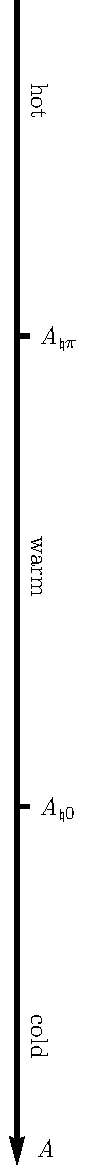
\includegraphics[height=13.6\textwidth]{bipolar-viable-arrow}
  \end{minipage}
  \begin{minipage}[b]{0.8\textwidth}
    \newcommand*{\legendtrimwidth}{0.03\textwidth}
    \newcommand*{\legendoffsetheight}{0.025\textwidth}
    
\includegraphics[
      width={\textwidth-\legendtrimwidth},
      trim={\legendtrimwidth} {-\legendoffsetheight} 0 0,
    ]{bipolar-viable-legend}
    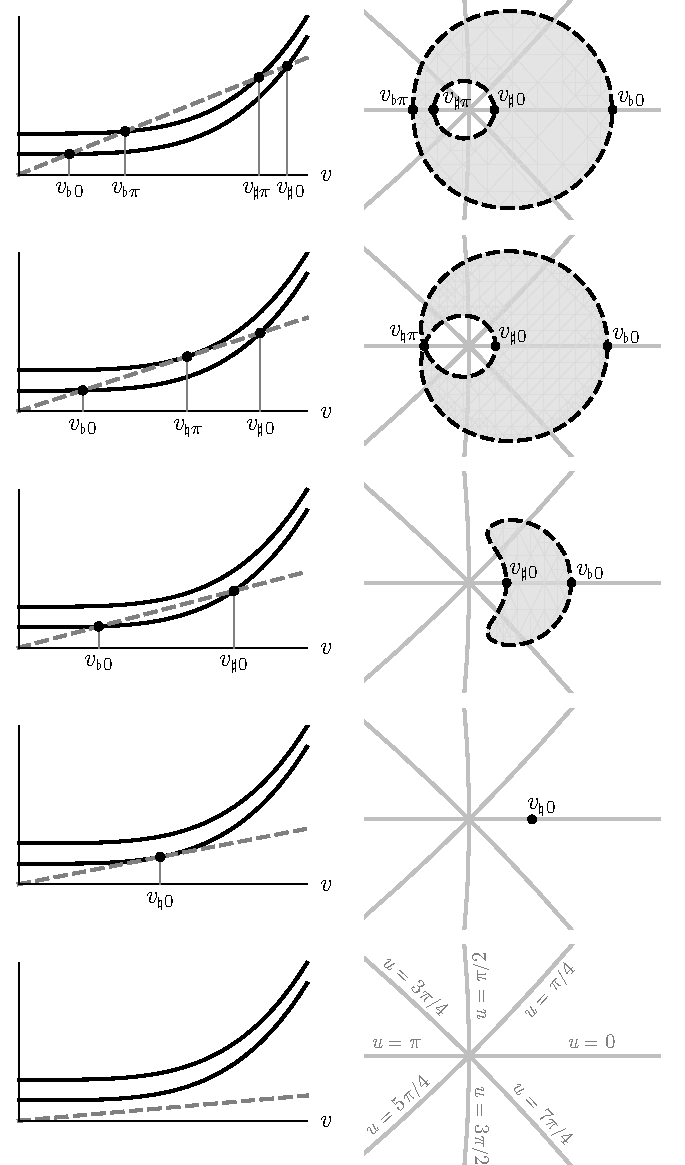
\includegraphics[width=\textwidth]{bipolar-viable}
  \end{minipage}
  \caption{
    Critical terminal points and non-viable domain~$\Phi < 0$
    for the known solution~(\ref{eq:bipolar-scaled-laplace-solution})
    and viability function~(\ref{eq:bipolar-viability-function}),
    as $A$~increases.
    In the right hand column,
    the $u$-contours~\figurestyle{grey curves} meet
    at the positive singularity~$v = +\infty$.
  }
  \label{fig:bipolar-viable}
\end{figure}

Each of~(\ref{eq:bipolar-critical-terminal-point-0})
and~(\ref{eq:bipolar-critical-terminal-point-pi})
has between zero and two roots
(ignoring~$v = 0$ for~(\ref{eq:bipolar-critical-terminal-point-0}))
depending on the size of the dimensionless group~$A$,
leading to five cases for the number of critical terminal points
and the geometry of the viable domain
(Figure~\ref{fig:bipolar-viable}):

\subsection{Five regimes}
\label{sec:bipolar.viable.regimes}

\begin{enumerate}
  \item
    \term{Hot regime}, $A < A_{\nat \pi}$:
    Both equations have two roots:
    $v_{\flat 0}$ and~$v_{\sharp 0}$
    for~(\ref{eq:bipolar-critical-terminal-point-0})
    and
    $v_{\flat \pi}$ and~$v_{\sharp \pi}$
    for~(\ref{eq:bipolar-critical-terminal-point-pi}),
    with~$v_{\flat 0} < v_{\flat \pi} < v_{\sharp \pi} < v_{\sharp 0}$.
    Thus there are four critical terminal points,
    having bipolar coordinates~$(0, v_{\flat 0})$, $(\pi, v_{\flat \pi})$,
    $(\pi, v_{\sharp \pi})$, and~$(0, v_{\sharp 0})$.
    The non-viable domain forms an avocado-like moat
    which surrounds an inner viable island
    (containing the singularity~$v = +\infty$)
    and is surrounded by an outer viable mainland.
  \item
    \term{Hot-to-warm transition}, $A = A_{\nat \pi}$:
    The two roots of~(\ref{eq:bipolar-critical-terminal-point-pi})
    merge together
    and the non-viable moat is pincered along~$u = \pi$,
    leaving the three critical terminal points~$(0, v_{\flat 0})$,
    $(\pi, v_{\nat \pi})$, and~$(0, v_{\sharp 0})$.
    The inner viable island and the outer viable mainland
    touch at the second of these.
  \item
    \term{Warm regime}, $A_{\nat \pi} < A < A_{\nat 0}$:
    The remaining root of~(\ref{eq:bipolar-critical-terminal-point-pi})
    has disappeared
    and the inner viable island is now robustly connected
    to the outer viable mainland.
    Equation~(\ref{eq:bipolar-critical-terminal-point-0}) still has two roots,
    corresponding to the two critical terminal points~%
      $(0, v_{\flat 0})$ and~$(0, v_{\sharp 0})$.
    The non-viable domain is now a crescent-shaped lake.
  \item
    \term{Warm-to-cold transition}, $A = A_{\nat 0}$:
    The two roots of~(\ref{eq:bipolar-critical-terminal-point-0})
    merge together
    and the non-viable lake dries up completely.
    The entire plane is viable,
    though a single (isolated) critical terminal point still exists
    at~$(0, v_{\nat 0})$.
  \item
    \term{Cold regime}, $A > A_{\nat 0}$:
    The last remaining root of~(\ref{eq:bipolar-critical-terminal-point-0})
    disappears.
    The entire plane is viable,
    and there are no critical terminal points left.
\end{enumerate}
The two transition cases occur
when~(\ref{eq:bipolar-critical-terminal-point-0})
and~(\ref{eq:bipolar-critical-terminal-point-pi})
each have a merging of roots,
at the special value of~$A$
for which the curves~$\cosh v \pm 1$ and~$v^4 / A$
touch tangentially,
given by the extra condition
\begin{equation}
  \sinh v - \frac{4 v^3}{A} = 0.
  \label{eq:bipolar-critical-terminal-point-transition}
\end{equation}
Note how this accounts for the situation in which
the terminal curve has an indeterminate local tangent
in equation~(\ref{eq:bipolar-terminal-curve-implicit-derivative}).
By numerically solving each of~(\ref{eq:bipolar-critical-terminal-point-0})
and~(\ref{eq:bipolar-critical-terminal-point-pi})
in conjunction with the tangency condition~%
  (\ref{eq:bipolar-critical-terminal-point-transition}),
the values of~$A$ for the two transitions are determined to be
\begin{align}
  A_{\nat \pi} &= 9.06433 \eqnspace \text{hot-to-warm},
    \label{eq:bipolar-transition-a-hot-to-warm}
    \\
  A_{\nat 0} &= 9.76206 \eqnspace \text{warm-to-cold}.
    \label{eq:bipolar-transition-a-warm-to-cold}
\end{align}

\section{Boundary tracing}
\label{sec:bipolar.tracing}

In this section we write down the boundary tracing ODE
and determine the class of convex domains which can be constructed.

\subsection{Candidate boundaries}
\label{sec:bipolar.tracing.candidates}

\begin{figure}
  \newcommand*{\subfigurewidth}{0.45\textwidth}
  \newcommand*{\subfigureoffsettop}{0.08\textwidth}
  \newcommand*{\subfigureoffsetbottom}{0.04\textwidth}
  \centering
  \begin{subfigure}{\subfigurewidth}
    \centredfigurecontent[
      trim=0 {\subfigureoffsetbottom} 0 0,
    ]{bipolar-traced-boundaries-hot}{Hot regime}
  \end{subfigure}
  \hfill
  \begin{subfigure}{\subfigurewidth}
    \centredfigurecontent[
      trim=0 {\subfigureoffsetbottom} 0 0,
    ]{bipolar-traced-boundaries-warm}{Warm regime}
  \end{subfigure}
  \begin{subfigure}{\subfigurewidth}
    \centredfigurecontent[
      trim=0 {\subfigureoffsetbottom} 0 {-\subfigureoffsettop},
    ]{bipolar-traced-boundaries-cold}{Cold regime}
  \end{subfigure}
  \caption{
    Traced boundaries obtained by integrating~%
      (\ref{eq:bipolar-tracing-ode-coordinate-parametrisation-v}).
  }
  \label{fig:bipolar-traced-boundaries}
\end{figure}

Using~(\ref{eq:bipolar-gradient-u-component})
through~(\ref{eq:bipolar-viability-function}),
the boundary tracing ODE~(\ref{eq:tracing-ode-coordinate-parametrisation-v})
becomes
\begin{important}{equation}
  \tder{v}{u} =
    \pm
    \frac{A}{v^4}
    \sqrt{
      \roundbr[\bulkysize]{\cosh v - \cos u}^2 - \frac{v^8}{A^2}
    },
  \label{eq:bipolar-tracing-ode-coordinate-parametrisation-v}
\end{important}
which cannot be integrated analytically.
Traced boundaries determined by numerical integration
from starting points in the viable domain
are shown in Figure~\ref{fig:bipolar-traced-boundaries}.

Like the line-source case of Section~\ref{sec:polar.tracing},
the two branches of traced boundaries are segregated
by the sign of~$\td v / {\td u}$,
with the upper branch spiralling inwards
and the lower branch spiralling outwards
as one travels anticlockwise
around the singularity~$v = +\infty$.
Again, any physically sensible radiation--conduction domain
must completely surround the heat-supplying singularity without touching it,
and therefore we seek closed curves surrounding the singularity,
made from patching together the traced boundaries
given by~(\ref{eq:bipolar-tracing-ode-coordinate-parametrisation-v}).
Using similar arguments to those in Section~\ref{sec:polar.tracing},
we conclude that a necessary (but not sufficient) condition
for the convexity of the sought-after closed curve
is for it to have an upper-to-lower branch switch
at an hyperbolic critical terminal point.

\begin{figure}
  \newcommand*{\subfigurewidth}{0.35\textwidth}
  \newcommand*{\subfigureoffsetbottom}{0.08\textwidth}
  \centering
  \hspace*{\fill}
  \begin{subfigure}{\subfigurewidth}
    \centredfigurecontent[
    ]{bipolar-critical-terminal-points-hot}{Hot regime}
  \end{subfigure}
    \hfill
  \begin{subfigure}{\subfigurewidth}
    \centredfigurecontent[
    ]{bipolar-critical-terminal-points-warm_hot}{Warm-to-hot transition}
  \end{subfigure}
  \hspace*{\fill}
  
  \hspace*{\fill}
  \begin{subfigure}{\subfigurewidth}
    \centredfigurecontent[
      trim=0 {\subfigureoffsetbottom} 0 0,
    ]{bipolar-critical-terminal-points-warm}{Warm regime}
  \end{subfigure}
    \hfill
  \begin{subfigure}{\subfigurewidth}
    \centredfigurecontent[
      trim=0 {\subfigureoffsetbottom} 0 0,
    ]{bipolar-critical-terminal-points-cold_warm}{Cold-to-warm transition}
  \end{subfigure}
  \hspace*{\fill}
  
  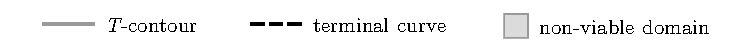
\includegraphics[
    width=\textwidth,
    trim=0 0 0 -5,
  ]{bipolar-critical-terminal-points-legend}
  \caption{
    Local $T$-contour through each critical terminal point.
  }
  \label{fig:critical-terminal-points}
\end{figure}

The nature of the up to four critical terminal points that exist
can be determined by inspecting Figure~\ref{fig:critical-terminal-points}.
We see that those lying on the segment~$u = \pi$
(to the left of the singularity)
are of elliptic type,
as the local $T$-contour lies on the non-viable side of the terminal curve.
Only the critical terminal points lying on the segment~$u = 0$
(to the right of the singularity)
are of hyperbolic type,
and it is from these points that we might construct convex domains.

\subsection{Convexity of the candidate boundaries}
\label{sec:bipolar.tracing.convex}

% TODO

\subsection{Numerical verification}
\label{sec:bipolar.tracing.verification}

% TODO

\section{Physical range}
\label{sec:bipolar.physical}

% TODO

\subsection{Temperature}
\label{sec:bipolar.physical.temperature}

% TODO

\subsection{Power per unit length}
\label{sec:bipolar.physical.power}

% TODO

\section{Summary}
\label{sec:bipolar.summary}

% TODO
